% Options for packages loaded elsewhere
\PassOptionsToPackage{unicode}{hyperref}
\PassOptionsToPackage{hyphens}{url}
%
\documentclass[
]{book}
\usepackage{amsmath,amssymb}
\usepackage{lmodern}
\usepackage{iftex}
\ifPDFTeX
  \usepackage[T1]{fontenc}
  \usepackage[utf8]{inputenc}
  \usepackage{textcomp} % provide euro and other symbols
\else % if luatex or xetex
  \usepackage{unicode-math}
  \defaultfontfeatures{Scale=MatchLowercase}
  \defaultfontfeatures[\rmfamily]{Ligatures=TeX,Scale=1}
\fi
% Use upquote if available, for straight quotes in verbatim environments
\IfFileExists{upquote.sty}{\usepackage{upquote}}{}
\IfFileExists{microtype.sty}{% use microtype if available
  \usepackage[]{microtype}
  \UseMicrotypeSet[protrusion]{basicmath} % disable protrusion for tt fonts
}{}
\makeatletter
\@ifundefined{KOMAClassName}{% if non-KOMA class
  \IfFileExists{parskip.sty}{%
    \usepackage{parskip}
  }{% else
    \setlength{\parindent}{0pt}
    \setlength{\parskip}{6pt plus 2pt minus 1pt}}
}{% if KOMA class
  \KOMAoptions{parskip=half}}
\makeatother
\usepackage{xcolor}
\usepackage{color}
\usepackage{fancyvrb}
\newcommand{\VerbBar}{|}
\newcommand{\VERB}{\Verb[commandchars=\\\{\}]}
\DefineVerbatimEnvironment{Highlighting}{Verbatim}{commandchars=\\\{\}}
% Add ',fontsize=\small' for more characters per line
\usepackage{framed}
\definecolor{shadecolor}{RGB}{248,248,248}
\newenvironment{Shaded}{\begin{snugshade}}{\end{snugshade}}
\newcommand{\AlertTok}[1]{\textcolor[rgb]{0.94,0.16,0.16}{#1}}
\newcommand{\AnnotationTok}[1]{\textcolor[rgb]{0.56,0.35,0.01}{\textbf{\textit{#1}}}}
\newcommand{\AttributeTok}[1]{\textcolor[rgb]{0.77,0.63,0.00}{#1}}
\newcommand{\BaseNTok}[1]{\textcolor[rgb]{0.00,0.00,0.81}{#1}}
\newcommand{\BuiltInTok}[1]{#1}
\newcommand{\CharTok}[1]{\textcolor[rgb]{0.31,0.60,0.02}{#1}}
\newcommand{\CommentTok}[1]{\textcolor[rgb]{0.56,0.35,0.01}{\textit{#1}}}
\newcommand{\CommentVarTok}[1]{\textcolor[rgb]{0.56,0.35,0.01}{\textbf{\textit{#1}}}}
\newcommand{\ConstantTok}[1]{\textcolor[rgb]{0.00,0.00,0.00}{#1}}
\newcommand{\ControlFlowTok}[1]{\textcolor[rgb]{0.13,0.29,0.53}{\textbf{#1}}}
\newcommand{\DataTypeTok}[1]{\textcolor[rgb]{0.13,0.29,0.53}{#1}}
\newcommand{\DecValTok}[1]{\textcolor[rgb]{0.00,0.00,0.81}{#1}}
\newcommand{\DocumentationTok}[1]{\textcolor[rgb]{0.56,0.35,0.01}{\textbf{\textit{#1}}}}
\newcommand{\ErrorTok}[1]{\textcolor[rgb]{0.64,0.00,0.00}{\textbf{#1}}}
\newcommand{\ExtensionTok}[1]{#1}
\newcommand{\FloatTok}[1]{\textcolor[rgb]{0.00,0.00,0.81}{#1}}
\newcommand{\FunctionTok}[1]{\textcolor[rgb]{0.00,0.00,0.00}{#1}}
\newcommand{\ImportTok}[1]{#1}
\newcommand{\InformationTok}[1]{\textcolor[rgb]{0.56,0.35,0.01}{\textbf{\textit{#1}}}}
\newcommand{\KeywordTok}[1]{\textcolor[rgb]{0.13,0.29,0.53}{\textbf{#1}}}
\newcommand{\NormalTok}[1]{#1}
\newcommand{\OperatorTok}[1]{\textcolor[rgb]{0.81,0.36,0.00}{\textbf{#1}}}
\newcommand{\OtherTok}[1]{\textcolor[rgb]{0.56,0.35,0.01}{#1}}
\newcommand{\PreprocessorTok}[1]{\textcolor[rgb]{0.56,0.35,0.01}{\textit{#1}}}
\newcommand{\RegionMarkerTok}[1]{#1}
\newcommand{\SpecialCharTok}[1]{\textcolor[rgb]{0.00,0.00,0.00}{#1}}
\newcommand{\SpecialStringTok}[1]{\textcolor[rgb]{0.31,0.60,0.02}{#1}}
\newcommand{\StringTok}[1]{\textcolor[rgb]{0.31,0.60,0.02}{#1}}
\newcommand{\VariableTok}[1]{\textcolor[rgb]{0.00,0.00,0.00}{#1}}
\newcommand{\VerbatimStringTok}[1]{\textcolor[rgb]{0.31,0.60,0.02}{#1}}
\newcommand{\WarningTok}[1]{\textcolor[rgb]{0.56,0.35,0.01}{\textbf{\textit{#1}}}}
\usepackage{longtable,booktabs,array}
\usepackage{calc} % for calculating minipage widths
% Correct order of tables after \paragraph or \subparagraph
\usepackage{etoolbox}
\makeatletter
\patchcmd\longtable{\par}{\if@noskipsec\mbox{}\fi\par}{}{}
\makeatother
% Allow footnotes in longtable head/foot
\IfFileExists{footnotehyper.sty}{\usepackage{footnotehyper}}{\usepackage{footnote}}
\makesavenoteenv{longtable}
\usepackage{graphicx}
\makeatletter
\def\maxwidth{\ifdim\Gin@nat@width>\linewidth\linewidth\else\Gin@nat@width\fi}
\def\maxheight{\ifdim\Gin@nat@height>\textheight\textheight\else\Gin@nat@height\fi}
\makeatother
% Scale images if necessary, so that they will not overflow the page
% margins by default, and it is still possible to overwrite the defaults
% using explicit options in \includegraphics[width, height, ...]{}
\setkeys{Gin}{width=\maxwidth,height=\maxheight,keepaspectratio}
% Set default figure placement to htbp
\makeatletter
\def\fps@figure{htbp}
\makeatother
\setlength{\emergencystretch}{3em} % prevent overfull lines
\providecommand{\tightlist}{%
  \setlength{\itemsep}{0pt}\setlength{\parskip}{0pt}}
\setcounter{secnumdepth}{5}
\usepackage{booktabs}
\ifLuaTeX
  \usepackage{selnolig}  % disable illegal ligatures
\fi
\usepackage[]{natbib}
\bibliographystyle{plainnat}
\IfFileExists{bookmark.sty}{\usepackage{bookmark}}{\usepackage{hyperref}}
\IfFileExists{xurl.sty}{\usepackage{xurl}}{} % add URL line breaks if available
\urlstyle{same} % disable monospaced font for URLs
\hypersetup{
  pdftitle={Congren's Notes},
  pdfauthor={Author: Congren Dai},
  hidelinks,
  pdfcreator={LaTeX via pandoc}}

\title{Congren's Notes}
\author{Author: Congren Dai}
\date{Last updated on 06 September, 2022}

\begin{document}
\maketitle

{
\setcounter{tocdepth}{1}
\tableofcontents
}
\hypertarget{linux-commands}{%
\chapter{Linux Commands}\label{linux-commands}}

This chapter contains \protect\hyperlink{basic}{basic commands} and \protect\hyperlink{advanced}{advanced commands} for Linux.

\hypertarget{basic}{%
\section{Basic Commands}\label{basic}}

\hypertarget{ls}{%
\subsection*{ls}\label{ls}}
\addcontentsline{toc}{subsection}{ls}

\begin{Shaded}
\begin{Highlighting}[]
\FunctionTok{ls} \CommentTok{\# list files}
\FunctionTok{ls} \AttributeTok{{-}l} \CommentTok{\# list files with permissions}
\FunctionTok{ls} \AttributeTok{{-}la} \CommentTok{\# list (hidden) files with permissions}
\end{Highlighting}
\end{Shaded}

\hypertarget{touch}{%
\subsection*{touch}\label{touch}}
\addcontentsline{toc}{subsection}{touch}

\begin{Shaded}
\begin{Highlighting}[]
\FunctionTok{touch}\NormalTok{ demo.txt }\CommentTok{\# create a file}
\FunctionTok{touch}\NormalTok{ demo1.txt demo2.txt demo3.txt }\CommentTok{\# create files}
\end{Highlighting}
\end{Shaded}

\hypertarget{mv}{%
\subsection*{mv}\label{mv}}
\addcontentsline{toc}{subsection}{mv}

\begin{Shaded}
\begin{Highlighting}[]
\FunctionTok{mv}\NormalTok{ demo.txt \textasciitilde{}/desktop }\CommentTok{\# move a file}
\FunctionTok{mv}\NormalTok{ demo.txt demo1.txt }\CommentTok{\# rename a file}
\FunctionTok{mv}\NormalTok{ demo.txt \textasciitilde{}/desktop/demo1.txt }\CommentTok{\# move and rename a file to a new place}
\end{Highlighting}
\end{Shaded}

\hypertarget{cat}{%
\subsection*{cat}\label{cat}}
\addcontentsline{toc}{subsection}{cat}

\begin{Shaded}
\begin{Highlighting}[]
\FunctionTok{cat}\NormalTok{ demo.txt }\CommentTok{\# see the content of a file}
\end{Highlighting}
\end{Shaded}

\hypertarget{head}{%
\subsection*{head}\label{head}}
\addcontentsline{toc}{subsection}{head}

\begin{Shaded}
\begin{Highlighting}[]
\FunctionTok{head}\NormalTok{ demo.txt }\CommentTok{\# check first 10 lines of the content}
\FunctionTok{head} \AttributeTok{{-}n}\NormalTok{ 20 demo.txt }\CommentTok{\# check 20 lines of the content}
\end{Highlighting}
\end{Shaded}

\hypertarget{tail}{%
\subsection*{tail}\label{tail}}
\addcontentsline{toc}{subsection}{tail}

\begin{Shaded}
\begin{Highlighting}[]
\FunctionTok{tail}\NormalTok{ demo.txt }\CommentTok{\# check last 10 lines of the content}
\FunctionTok{tail} \AttributeTok{{-}n}\NormalTok{ 20 demo.txt }\CommentTok{\# check 20 lines of the content}
\FunctionTok{tail} \AttributeTok{{-}f}\NormalTok{ demo.txt }\CommentTok{\# check the added content to the file consistently}
\end{Highlighting}
\end{Shaded}

One example of using ``tail -f'' is when you want to check a log file.

\hypertarget{mkdir}{%
\subsection*{mkdir}\label{mkdir}}
\addcontentsline{toc}{subsection}{mkdir}

\begin{Shaded}
\begin{Highlighting}[]
\FunctionTok{mkdir}\NormalTok{ demo }\CommentTok{\# make a directory}
\FunctionTok{mkdir} \AttributeTok{{-}p}\NormalTok{ demo1/demo2/demo3/demo4 }\CommentTok{\# make a directory recursively}
\end{Highlighting}
\end{Shaded}

\hypertarget{rm}{%
\subsection*{rm}\label{rm}}
\addcontentsline{toc}{subsection}{rm}

\begin{Shaded}
\begin{Highlighting}[]
\FunctionTok{rm}\NormalTok{ demo.txt }\CommentTok{\# delete a file}
\FunctionTok{rm} \AttributeTok{{-}rf}\NormalTok{ demo }\CommentTok{\# delete a directory  }
\FunctionTok{rm} \AttributeTok{{-}rf}\NormalTok{ demo1 demo2 demo3 }\CommentTok{\# delete more than one directory.}
\FunctionTok{rm}\NormalTok{ demo1.txt demo2.txt demo3.txt }\CommentTok{\# delete more than one file}
\end{Highlighting}
\end{Shaded}

\hypertarget{cp}{%
\subsection*{cp}\label{cp}}
\addcontentsline{toc}{subsection}{cp}

\begin{Shaded}
\begin{Highlighting}[]
\FunctionTok{cp}\NormalTok{ demo.txt \textasciitilde{}/desktop/ }\CommentTok{\# copy a file to the desktop }
\FunctionTok{cp}\NormalTok{ demo.txt \textasciitilde{}/desktop/demo1.txt }\CommentTok{\# copy a file and rename it}
\FunctionTok{cp} \AttributeTok{{-}r}\NormalTok{ demo1 \textasciitilde{}/desktop/demo1 }\CommentTok{\# copy a directory and rename it}
\end{Highlighting}
\end{Shaded}

\hypertarget{tar}{%
\subsection*{tar}\label{tar}}
\addcontentsline{toc}{subsection}{tar}

\begin{Shaded}
\begin{Highlighting}[]
\FunctionTok{tar} \AttributeTok{{-}zcvf}\NormalTok{ demo.tar.gz ./demo.txt }\CommentTok{\# create an archive (file)}
\FunctionTok{tar} \AttributeTok{{-}zcvf}\NormalTok{ demo.tar.gz ./demo }\CommentTok{\# create an archive (directory)}
\FunctionTok{tar} \AttributeTok{{-}zxvf}\NormalTok{ demo.tar.gz }\CommentTok{\# uncompress an archive}
\FunctionTok{tar} \AttributeTok{{-}zxvf}\NormalTok{ demo.tar.gz }\AttributeTok{{-}C}\NormalTok{ ./Aaron }\CommentTok{\# uncompress and rename an archive}
\FunctionTok{tar} \AttributeTok{{-}tf}\NormalTok{ demo.tar.gz }\CommentTok{\# see the files in an archive}
\end{Highlighting}
\end{Shaded}

A .tar file creates an archive without compressing\\
A .gz (gzip) file compresses files without creating an archive\\
A .tar.gz file archives and compresses multiple files into one\\
-z: use gzip\\
-c: create archives\\
-v: display information (not necessary to use)\\
-f: creates archives with given filename\\
-C: uncompress archives to a specific place

\hypertarget{find}{%
\subsection*{find}\label{find}}
\addcontentsline{toc}{subsection}{find}

\begin{Shaded}
\begin{Highlighting}[]
\FunctionTok{find}\NormalTok{ / }\AttributeTok{{-}name}\NormalTok{ demo.txt }\CommentTok{\# find a file from the root}
\FunctionTok{find}\NormalTok{ \textasciitilde{}/desktop }\AttributeTok{{-}name}\NormalTok{ demo.txt }\CommentTok{\# find a file from the desktop}
\FunctionTok{find}\NormalTok{ / }\AttributeTok{{-}name}\NormalTok{ demo}\PreprocessorTok{*} \CommentTok{\# find any file that starts with demo from the root directory}
\FunctionTok{find}\NormalTok{ / }\AttributeTok{{-}name} \PreprocessorTok{*}\NormalTok{.txt }\CommentTok{\# find any file that ends with .txt from the root directory}
\end{Highlighting}
\end{Shaded}

If you are using macOS, you have to change the command to find / -name `demo.txt'.

\hypertarget{advanced}{%
\section{Advanced Commands}\label{advanced}}

\hypertarget{ps}{%
\subsection*{ps}\label{ps}}
\addcontentsline{toc}{subsection}{ps}

\begin{Shaded}
\begin{Highlighting}[]

\end{Highlighting}
\end{Shaded}

\hypertarget{grep}{%
\subsection*{grep}\label{grep}}
\addcontentsline{toc}{subsection}{grep}

\begin{Shaded}
\begin{Highlighting}[]

\end{Highlighting}
\end{Shaded}

\citet{xie2015}

\hypertarget{matplotlib}{%
\chapter{Matplotlib}\label{matplotlib}}

There are three Matplotlib cheatsheets for beginners (Figure \ref{fig:beginner}), intermediate users (Figure \ref{fig:intermediate}), and some tips and tricks (Figure \ref{fig:tips}).

\url{https://matplotlib.org/cheatsheets/}

\hypertarget{beginners}{%
\section{Beginners}\label{beginners}}

\begin{figure}

{\centering 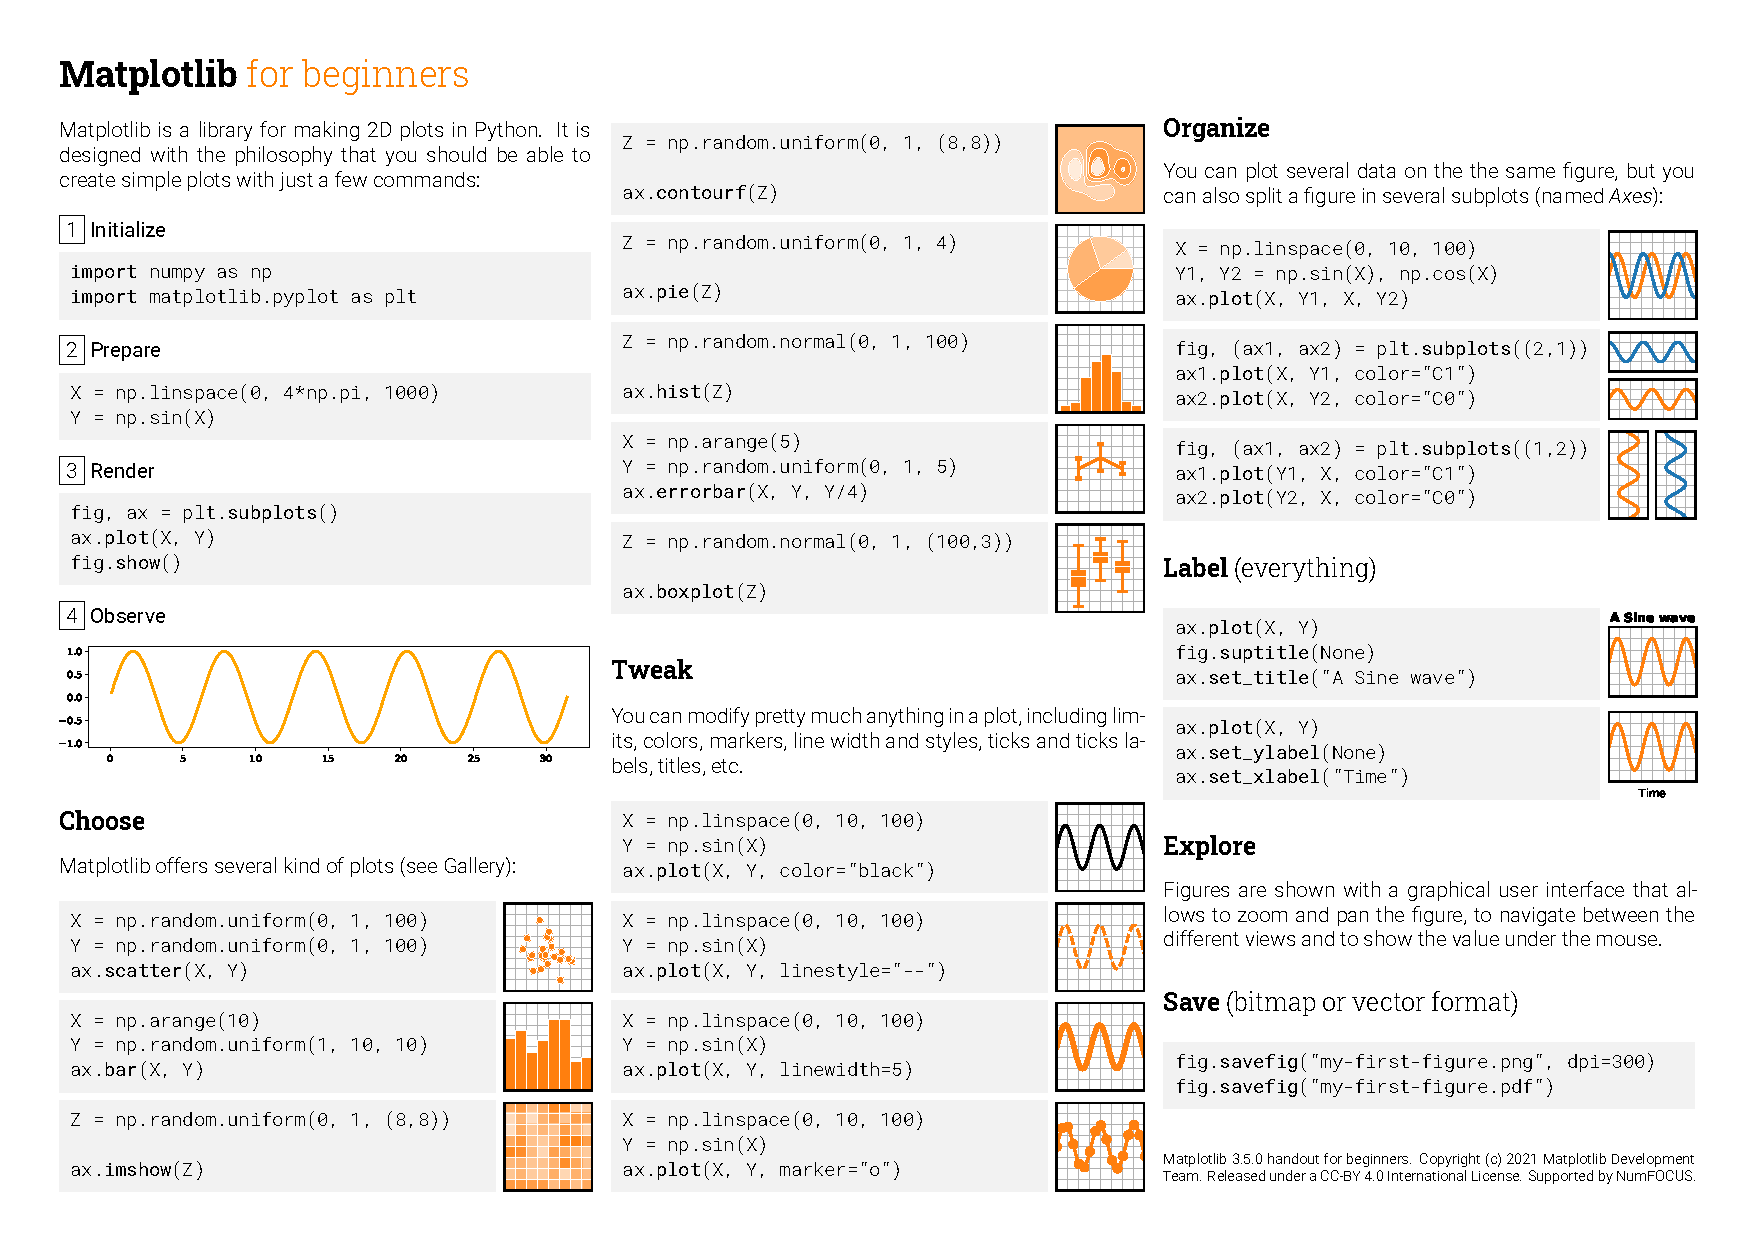
\includegraphics[width=1\linewidth]{matplotlib/handout-beginner} 

}

\caption{Matplotlib for beginners}\label{fig:beginner}
\end{figure}

\hypertarget{intermediate-users}{%
\section{Intermediate users}\label{intermediate-users}}

\begin{figure}

{\centering 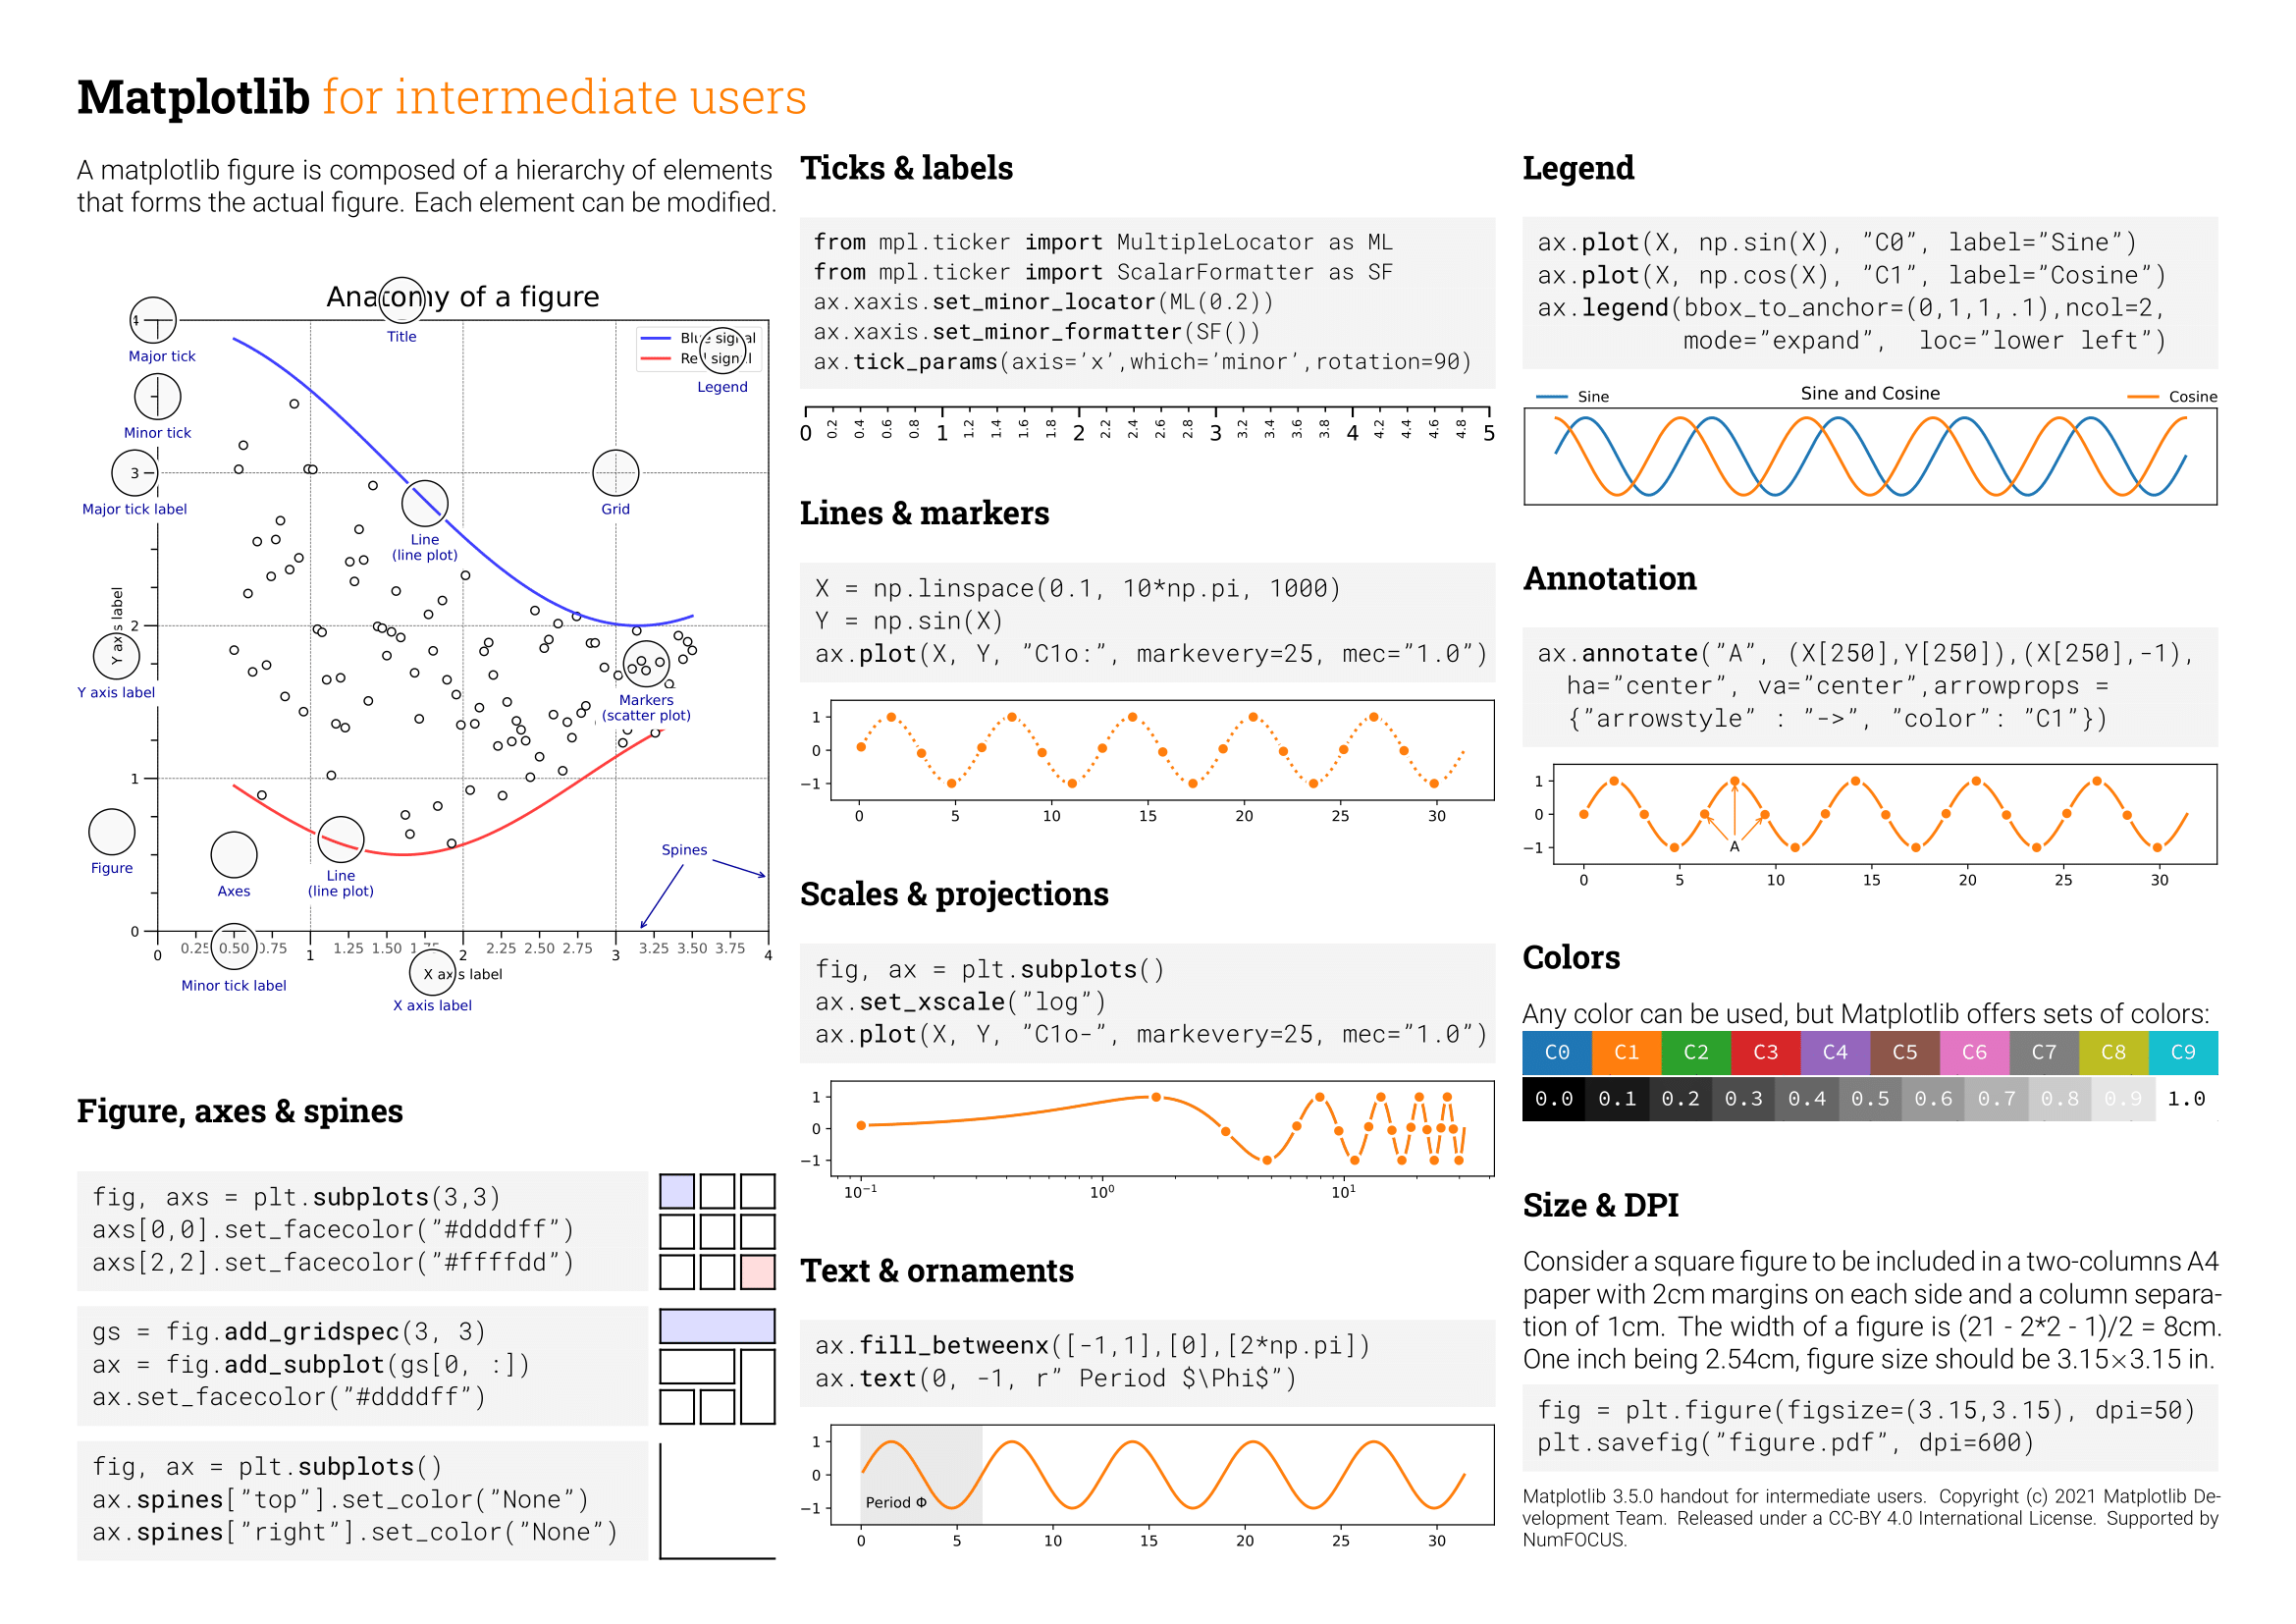
\includegraphics[width=1\linewidth]{matplotlib/handout-intermediate} 

}

\caption{Matplotlib for intermediate users}\label{fig:intermediate}
\end{figure}

\hypertarget{tips-tricks}{%
\section{Tips \& Tricks}\label{tips-tricks}}

\begin{figure}

{\centering 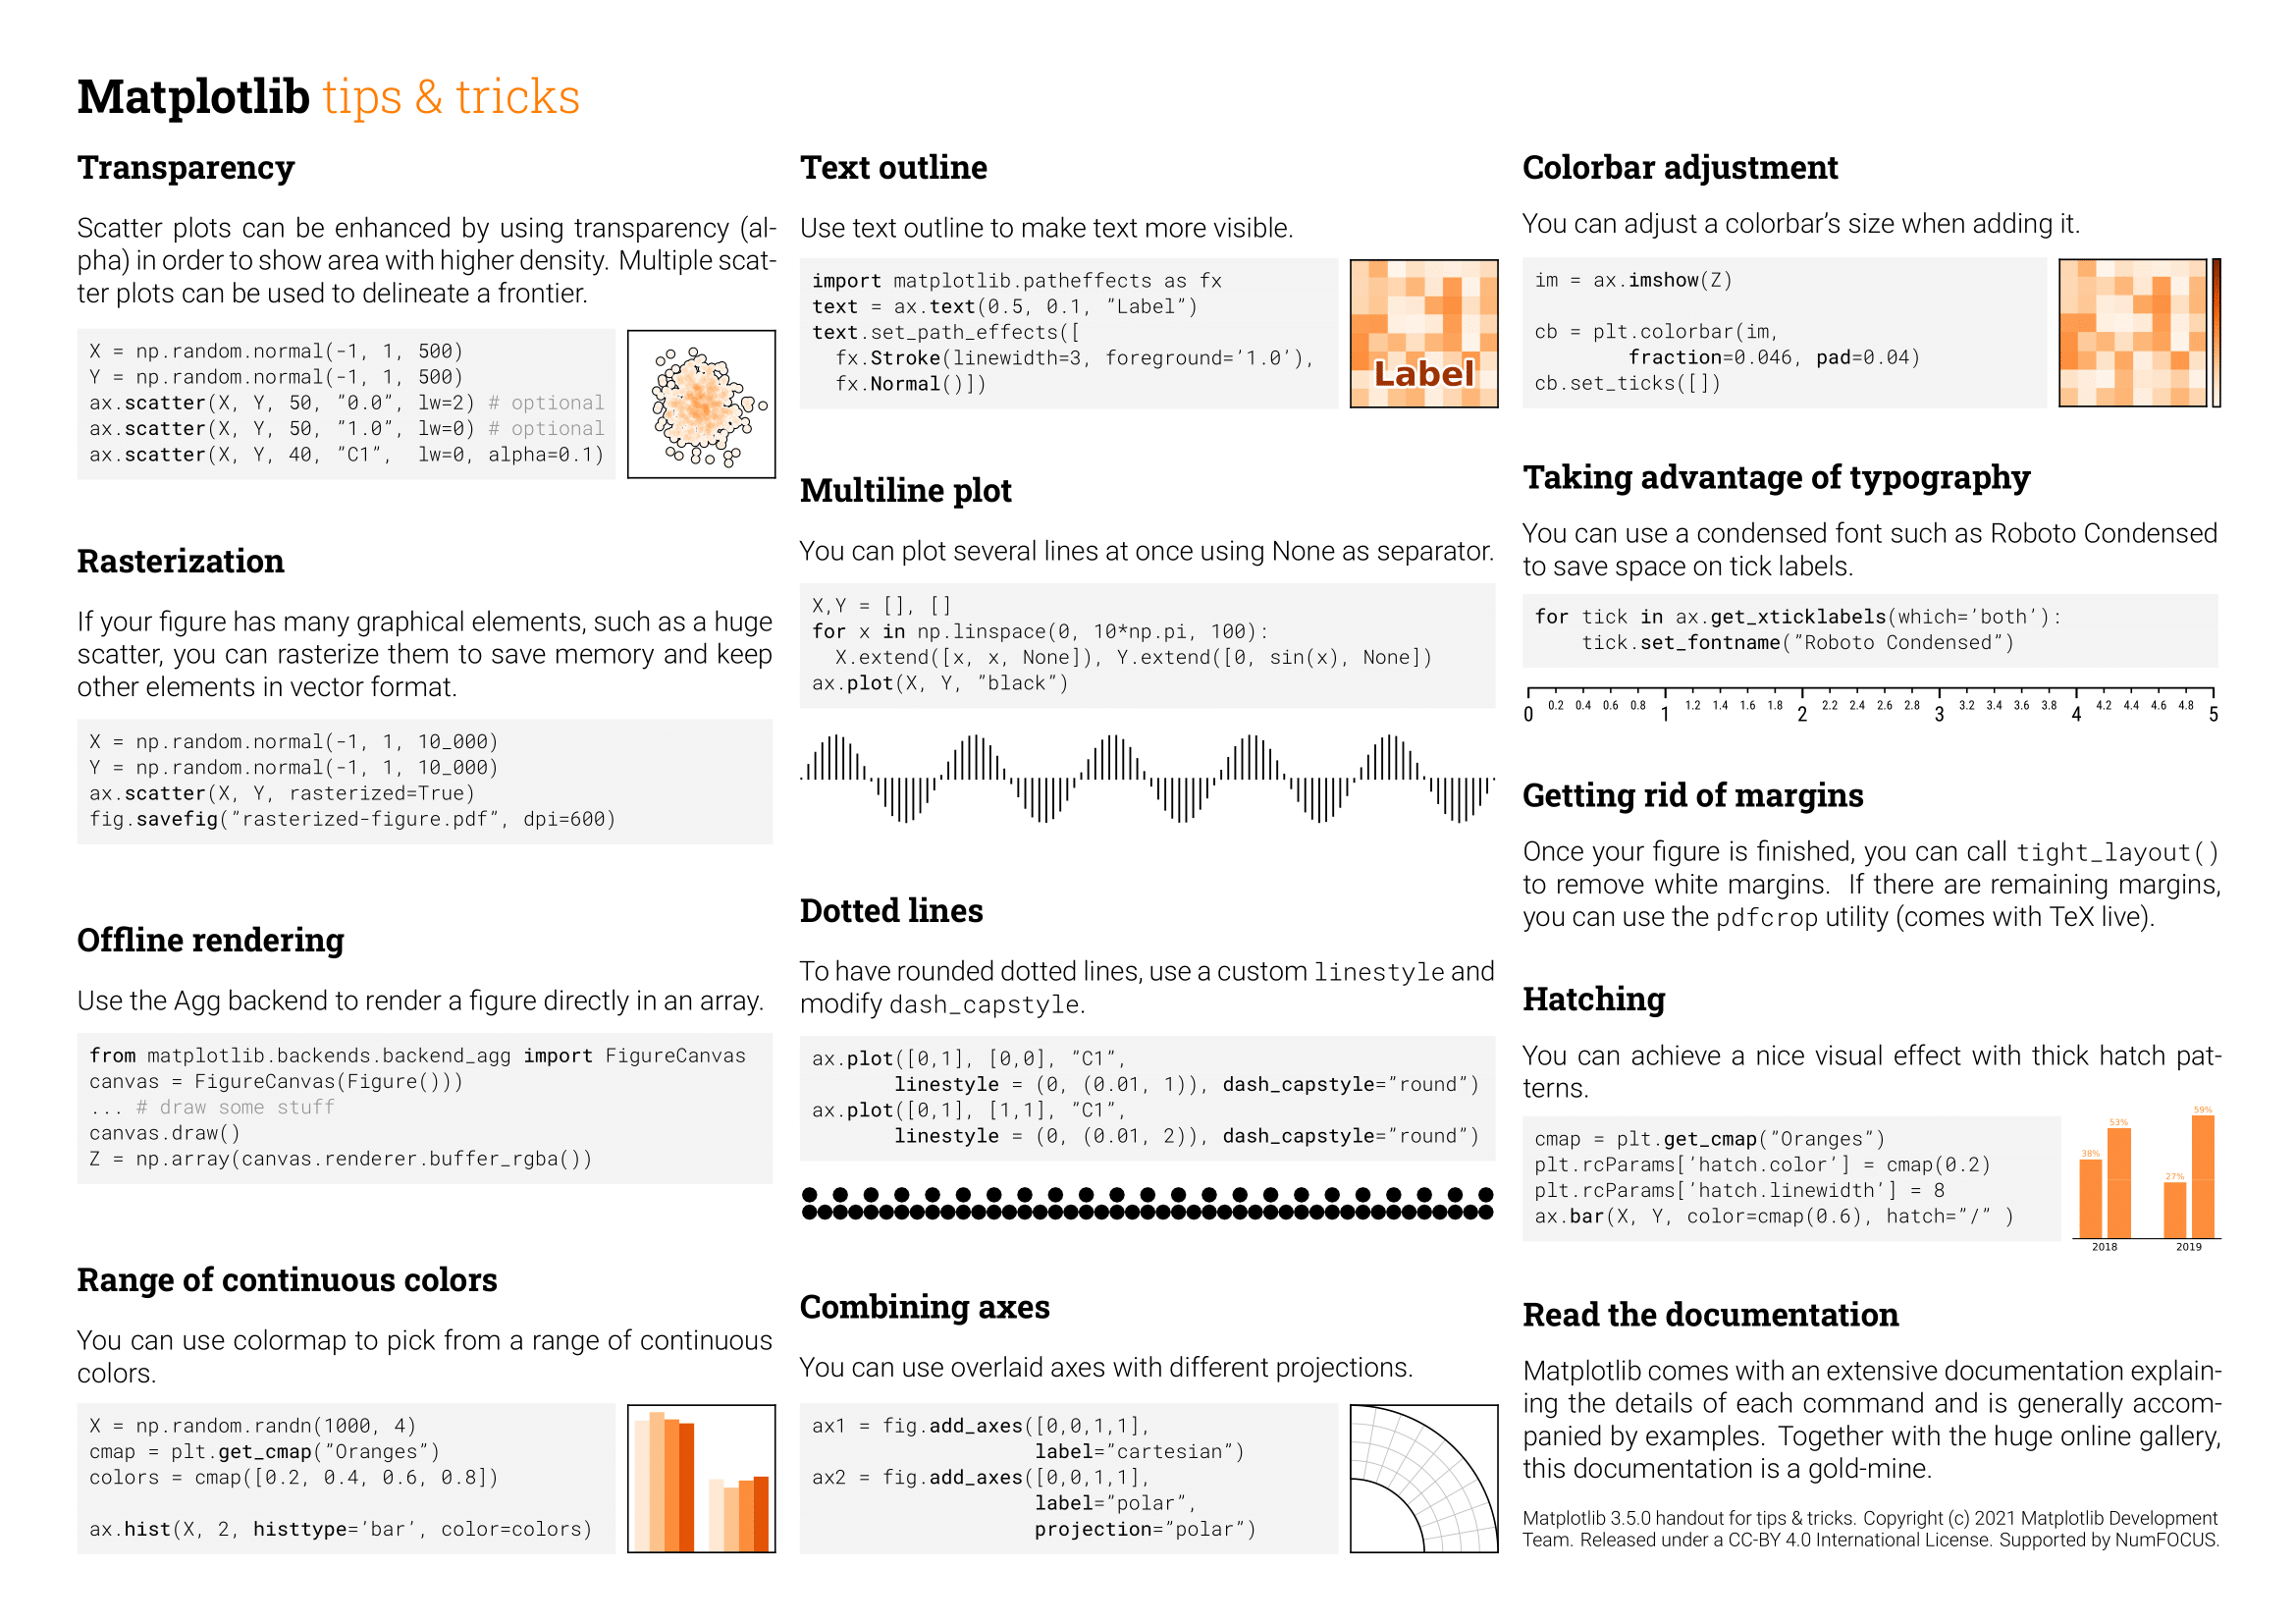
\includegraphics[width=1\linewidth]{matplotlib/handout-tips} 

}

\caption{Matplotlib tips and tricks}\label{fig:tips}
\end{figure}

  \bibliography{book.bib,packages.bib}

\end{document}
